\documentclass[10pt]{article}
\usepackage[polish]{babel}
\usepackage[utf8]{inputenc}
\usepackage[T1]{fontenc}
\usepackage{amsmath}
\usepackage{amsfonts}
\usepackage{amssymb}
\usepackage[version=4]{mhchem}
\usepackage{stmaryrd}
\usepackage{graphicx}
\usepackage[export]{adjustbox}
\graphicspath{ {./images/} }

\title{XV Konkurs Matematyczny St@ś }

\author{}
\date{}


\begin{document}
\maketitle
XIV LO im. Stanisława Staszica\\
25 maja 2015 roku

\section*{klasa VI}
Na rozwiazanie poniższych zadań masz 90 minut. Kolejność rozwiazywania tych zadań jest dowolna. Wszystkie zadania sa jednakowo punktowane. Maksymalna liczbę punktów może uzyskać jedynie petne rozwiazanie, z uzasadnieniem \(\boldsymbol{i}\) odpowiedzia.\\
Używanie korektora i korzystanie z kalkulatora jest niedozwolone.

\begin{enumerate}
  \item Dzieląc pewną liczbę naturalną \(n\) przez 60 otrzymujemy iloraz 17 i resztę 55 . Oblicz iloraz i resztę z dzielenia liczby \(n\) przez 15 .
  \item Ile jest dziesięciocyfrowych liczb o sumie cyfr równej 3.
  \item Dany jest trapez równoramienny \(A B C D\) o podstawach \(A B\) i \(C D\). Na przedłużeniu boku \(A B\) poza punkt \(B\) wybrano taki punkt \(E\), że \(B E=C D\). Udowodnij, że odcinki \(A C\) i \(E C\) mają równą długość.\\
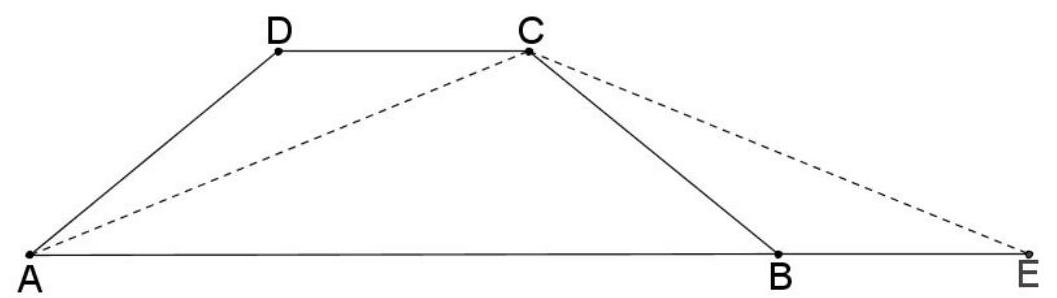
\includegraphics[max width=\textwidth, center]{2024_11_21_dbc9ac1df4a08138bbc0g-1}
  \item Staś wybrał pewną liczbę naturalną \(a\). Okazało się, że spełnia ona następującą równość:
\end{enumerate}

\[
3\left(a^{2}+3 a\right)=194 \square
\]

Wyznacz brakującą cyfrę jedności.\\
5. Staś napisał na tablicy liczby naturalne \(1,2,3\). W jednym ruchu może zetrzeć dowolną z napisanych liczb i zamiast niej napisać liczbę będącą sumą lub różnicą dwóch pozostałych. Czy po pewnej liczbie takich ruchów na tablicy może pojawić się trójka liczb:\\
966, 1410 i 2376 ?


\end{document}